% Options for packages loaded elsewhere
\PassOptionsToPackage{unicode}{hyperref}
\PassOptionsToPackage{hyphens}{url}
%
\documentclass[
]{article}
\title{Travail de session BOT500 - Une abondance d'oiseaux du Nord au
Sud du Québec}
\author{Frédérick St-Pierre \and Yohan Wegener \and Félix
Labbé \and Aurel Veillet}
\date{2024-04-24}

\usepackage{amsmath,amssymb}
\usepackage{lmodern}
\usepackage{iftex}
\ifPDFTeX
  \usepackage[T1]{fontenc}
  \usepackage[utf8]{inputenc}
  \usepackage{textcomp} % provide euro and other symbols
\else % if luatex or xetex
  \usepackage{unicode-math}
  \defaultfontfeatures{Scale=MatchLowercase}
  \defaultfontfeatures[\rmfamily]{Ligatures=TeX,Scale=1}
\fi
% Use upquote if available, for straight quotes in verbatim environments
\IfFileExists{upquote.sty}{\usepackage{upquote}}{}
\IfFileExists{microtype.sty}{% use microtype if available
  \usepackage[]{microtype}
  \UseMicrotypeSet[protrusion]{basicmath} % disable protrusion for tt fonts
}{}
\makeatletter
\@ifundefined{KOMAClassName}{% if non-KOMA class
  \IfFileExists{parskip.sty}{%
    \usepackage{parskip}
  }{% else
    \setlength{\parindent}{0pt}
    \setlength{\parskip}{6pt plus 2pt minus 1pt}}
}{% if KOMA class
  \KOMAoptions{parskip=half}}
\makeatother
\usepackage{xcolor}
\IfFileExists{xurl.sty}{\usepackage{xurl}}{} % add URL line breaks if available
\IfFileExists{bookmark.sty}{\usepackage{bookmark}}{\usepackage{hyperref}}
\hypersetup{
  pdftitle={Travail de session BOT500 - Une abondance d'oiseaux du Nord au Sud du Québec},
  pdfauthor={Frédérick St-Pierre; Yohan Wegener; Félix Labbé; Aurel Veillet},
  hidelinks,
  pdfcreator={LaTeX via pandoc}}
\urlstyle{same} % disable monospaced font for URLs
\usepackage[margin=1in]{geometry}
\usepackage{graphicx}
\makeatletter
\def\maxwidth{\ifdim\Gin@nat@width>\linewidth\linewidth\else\Gin@nat@width\fi}
\def\maxheight{\ifdim\Gin@nat@height>\textheight\textheight\else\Gin@nat@height\fi}
\makeatother
% Scale images if necessary, so that they will not overflow the page
% margins by default, and it is still possible to overwrite the defaults
% using explicit options in \includegraphics[width, height, ...]{}
\setkeys{Gin}{width=\maxwidth,height=\maxheight,keepaspectratio}
% Set default figure placement to htbp
\makeatletter
\def\fps@figure{htbp}
\makeatother
\setlength{\emergencystretch}{3em} % prevent overfull lines
\providecommand{\tightlist}{%
  \setlength{\itemsep}{0pt}\setlength{\parskip}{0pt}}
\setcounter{secnumdepth}{-\maxdimen} % remove section numbering
\ifLuaTeX
  \usepackage{selnolig}  % disable illegal ligatures
\fi

\begin{document}
\maketitle

{
\setcounter{tocdepth}{2}
\tableofcontents
}
Significance: ``Ce travail a été réalisé dans le cadre du cours BOT500
par des étudiants au BAC en écologie.''

keywords: - ``Diversité'' - ``Paruline'' - ``Québec''

pnas\_type: pnasresearcharticle bibliography: pnas-sample.bib csl:
pnas.csl lineno: false --- \#\# Résumé ``This study investigates the
abundance of birds from Northern to Southern Quebec. We analyze the
distribution patterns of various bird species and assess their diversity
across different ecological regions. Our findings highlight the
importance of conservation efforts in preserving avian biodiversity in
Quebec.''

\hypertarget{introduction}{%
\subsection{Introduction}\label{introduction}}

``Afin de comprendre la dynamique de la biodiversité aviaire du Québec
sur une période donnée, nous avons établi une question générale composée
de deux sous-questions nous permettant d'y parvenir: Y a-t-il une
corrélation entre la richesse spécifique et l'abondance des espèces
d'oiseaux au Québec? Quelle est la tendance de la richesse aviaire
spécifique du Québec de 2016 à 2020? Quelle est la tendance d'abondance
selon la latitude?

La première question cherche à établir s'il existe une corrélation entre
la richesse spécifique (le nombre total d'espèces) et l'abondance (la
quantité relative de chaque espèce). Comprendre cette relation est
crucial pour évaluer la santé globale d'un écosystème et comment il
pourrait être affecté par des changements environnementaux.

La deuxième question cherche à analyser la tendance de la richesse
aviaire spécifique dans la région du Québec au cours des années 2016 à
2020. Cette analyse temporelle permettrait de détecter des changements
survenus dans la diversité des espèces aviaires au fil du temps, ce qui
pourrait être lié à des facteurs tels que le changement climatique, la
dégradation de l'habitat ou d'autres pressions environnementales.

Enfin, la troisième question explore la variabilité saisonnière de la
richesse aviaire spécifique. La diversité des espèces aviaires varie
tout au long de l'année à la suite des changements de saison. Les
résultats peuvent fournir des informations importantes sur les schémas
de migration, les cycles de reproduction et les fluctuations des
populations, ce qui est crucial pour la conservation et la gestion des
écosystèmes. En somme, ces questions cherchent à éclairer les liens
complexes entre la biodiversité aviaire, le temps et l'environnement
dans la région du Québec.''

\hypertarget{muxe9thode}{%
\subsection{Méthode}\label{muxe9thode}}

``Les données utilisées dans ce travail représentent la composition et
la phénologie sonore des oiseaux au Québec, recueillies dans le cadre
d'un programme de surveillance de la biodiversité acoustique mené par le
ministère de l'Environnement, de la Lutte contre les Changements
Climatiques, de la Faune et des Parcs (MELCCFP), dans le contexte du
Réseau de suivi de la biodiversité du Québec. Elles répertorient les
observations sonores des oiseaux. Les inventaires acoustiques sont
réalisés au moyen d'enregistreurs sonores qui capturent les cris et les
chants des oiseaux. Ces enregistrements représentent des efforts
d'échantillonnage et sont ensuite analysés par un spécialiste en
taxonomie qui identifie les espèces d'oiseaux enregistrées. Lorsque
possible, l'heure de l'observation est également enregistrée
(time\_obs). Ainsi, ces données ont été analysées grâce au logiciel R
afin de créer des figures qui représentent les résultats correspondant
aux trois questions énoncées ci-dessus.''

\hypertarget{ruxe9sultats}{%
\subsection{Résultats}\label{ruxe9sultats}}

``À la suite de la création d'une base de données et des analyses dans
RStudio, trois figures ont été créées afin de mieux répondre à nos
questions.''

\begin{itemize}
\item
  La Figure 1 présente le nombre d'espèces présentes en fonction de la
  latitude du Québec. La régression en bleu permet de voir la moyenne
  d'espèces uniques. Les points présents dans la figure représentent
  chaque station d'écoute.
\item
  La Figure 2 présente l'abondance des observations de parulines, elle
  aussi en fonction de la latitude. Une régression, en bleu, avec
  l'incertitude, en gris, est observable.
\item
  La Figure 3 présente le nombre d'espèces uniques observées dans tous
  les sites d'échantillonnages de l'étude pour chaque année, de 2016 à
  2020.''
\item
  La figure 4 présente
\end{itemize}

\begin{figure}
\centering
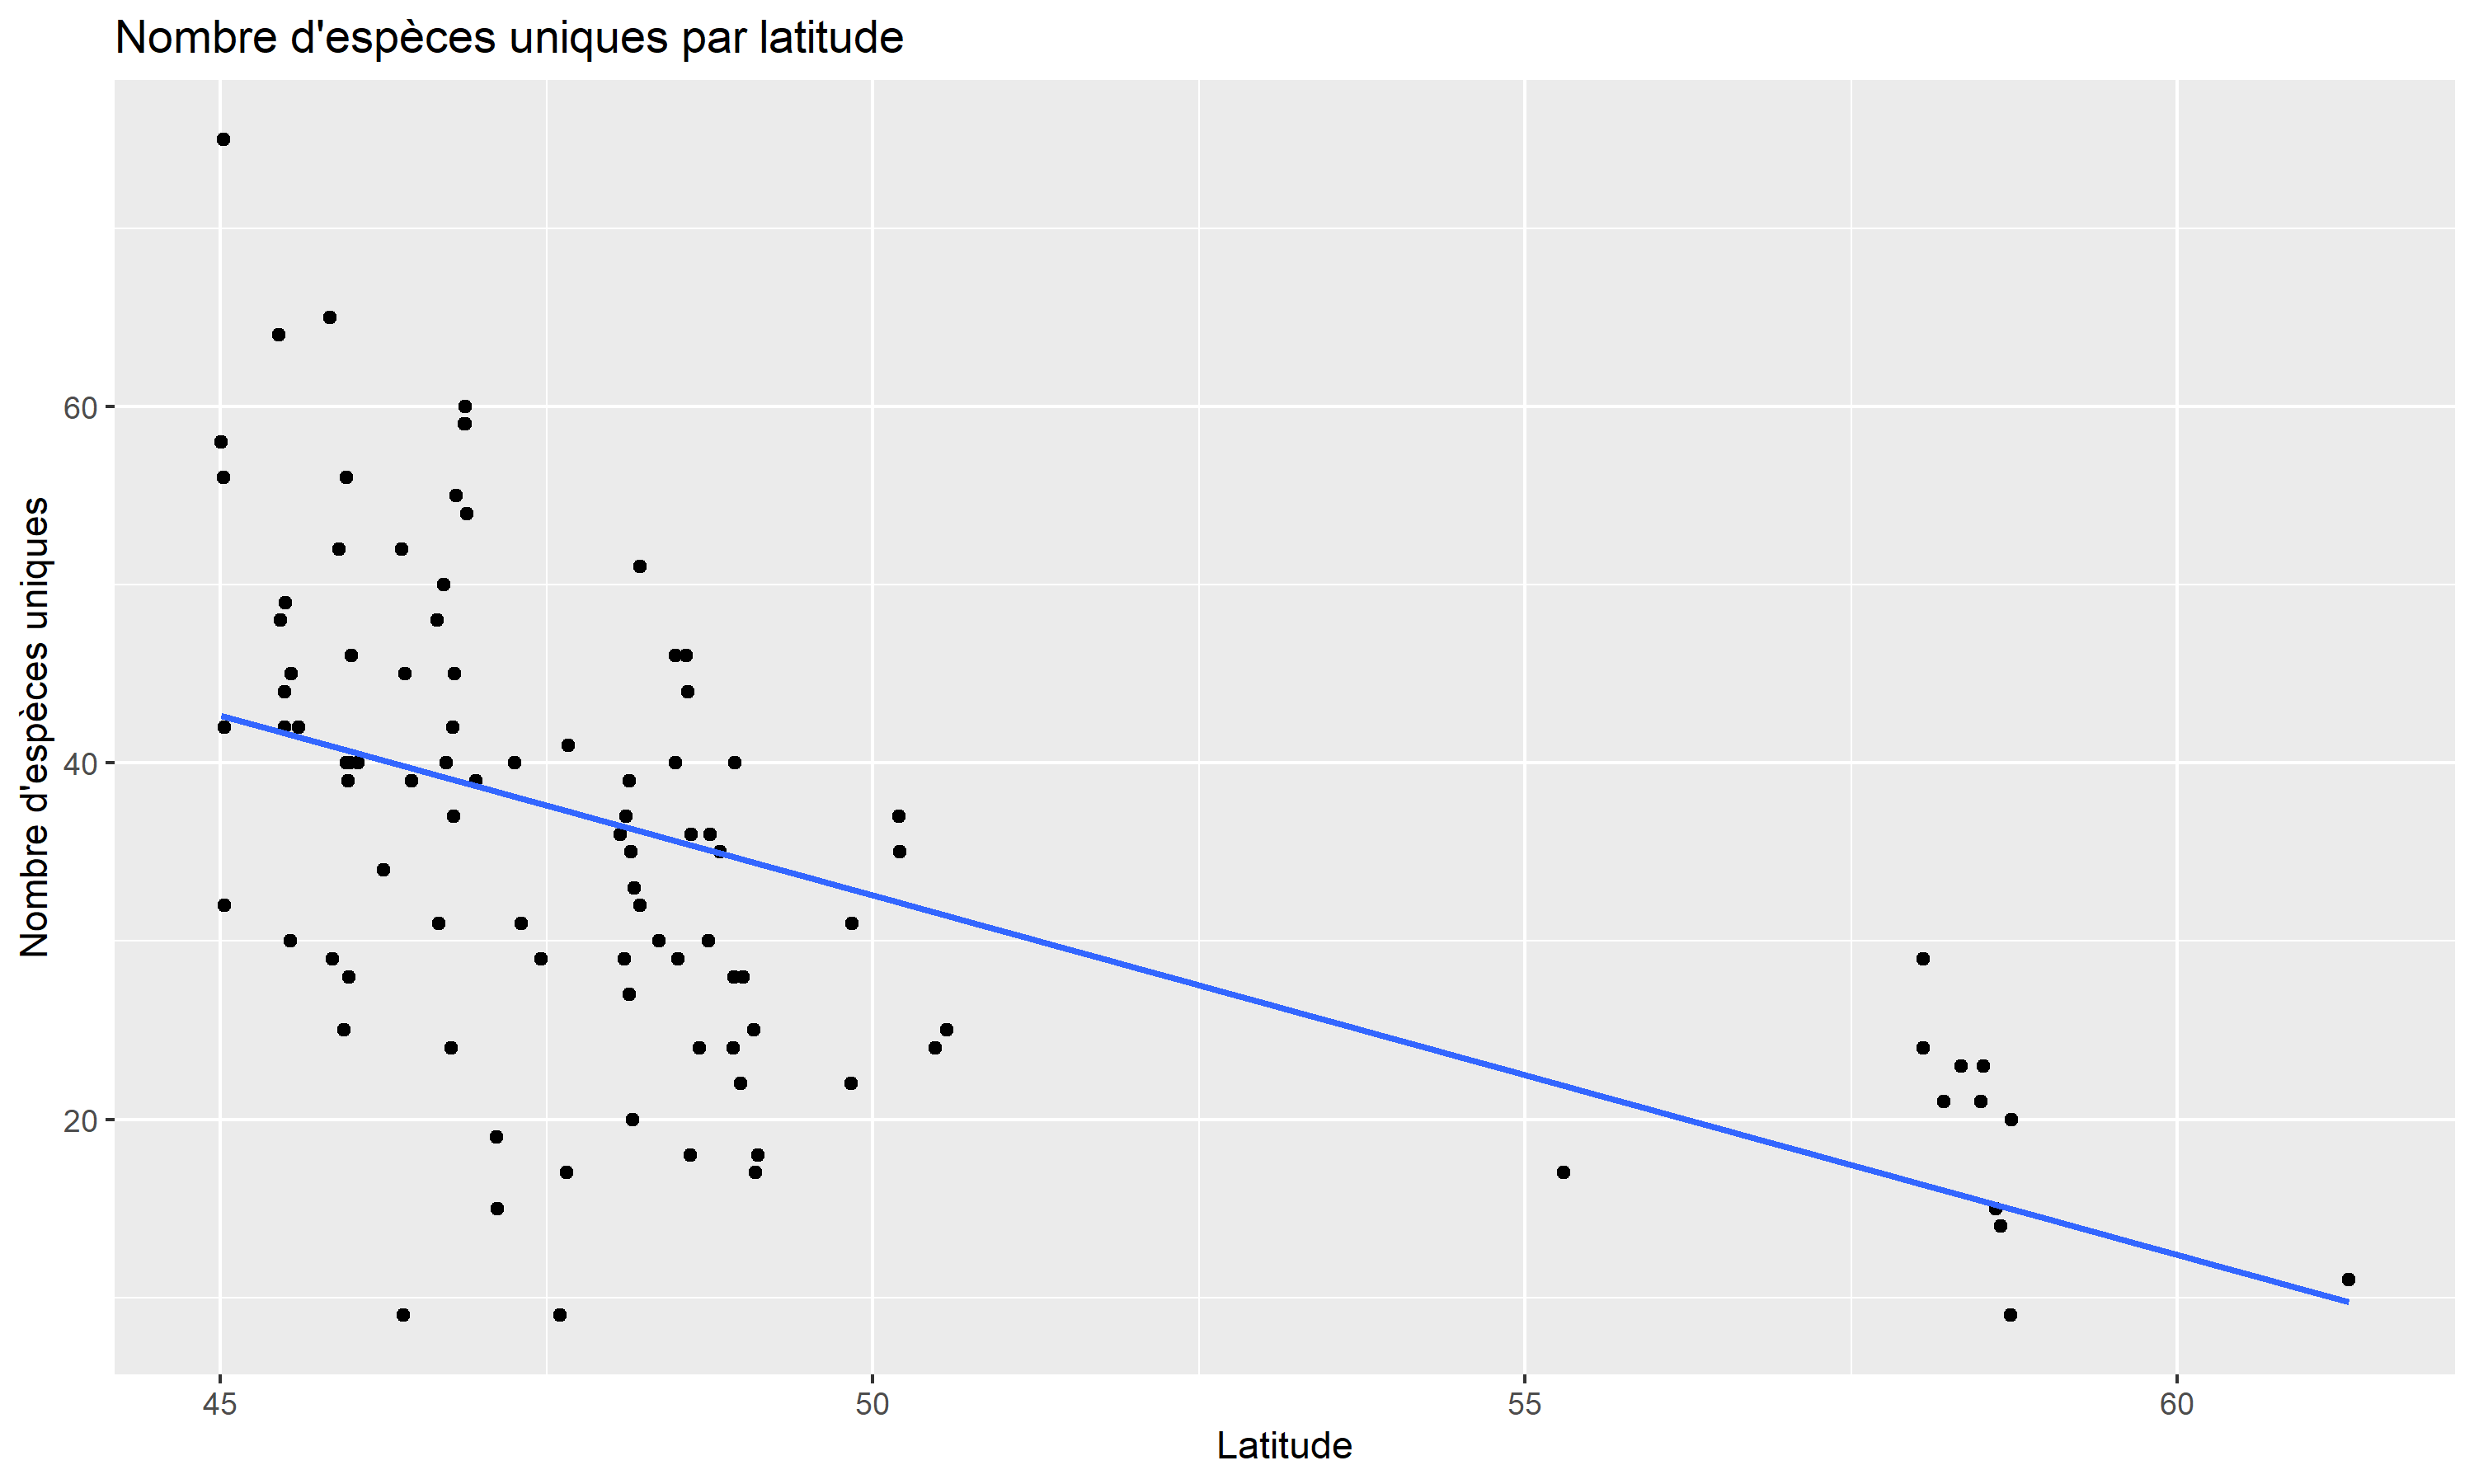
\includegraphics{/rapport/Fig1.png}
\caption{Figure 1: Nombre d'espèce en fonction de la latitude au Québec}
\end{figure}

\begin{figure}
\centering
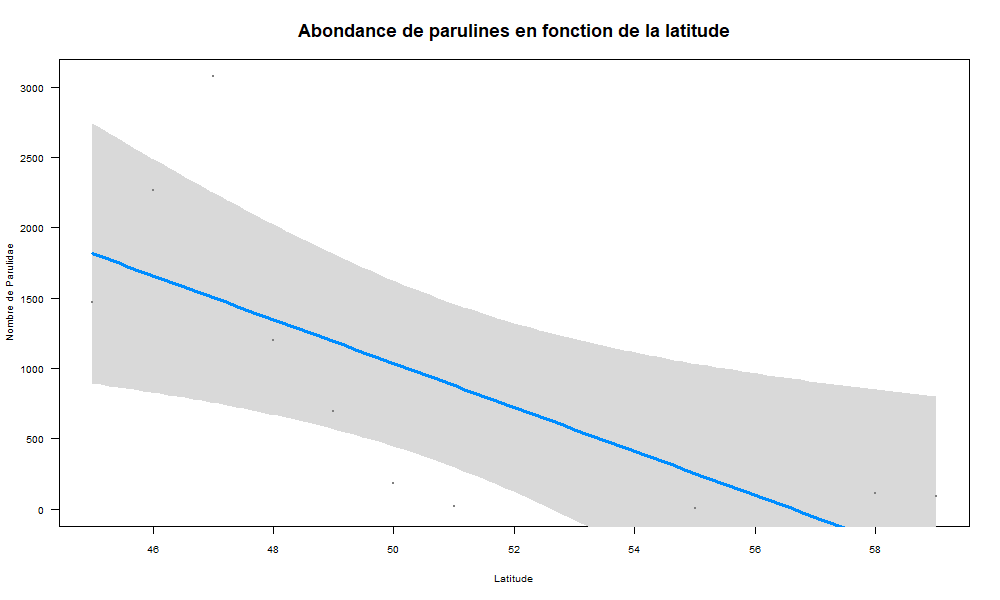
\includegraphics{./rapport/Figure2.png}
\caption{Figure 2: Abondance de paruline en fonction de la latitude au
Québec}
\end{figure}

\begin{figure}
\centering
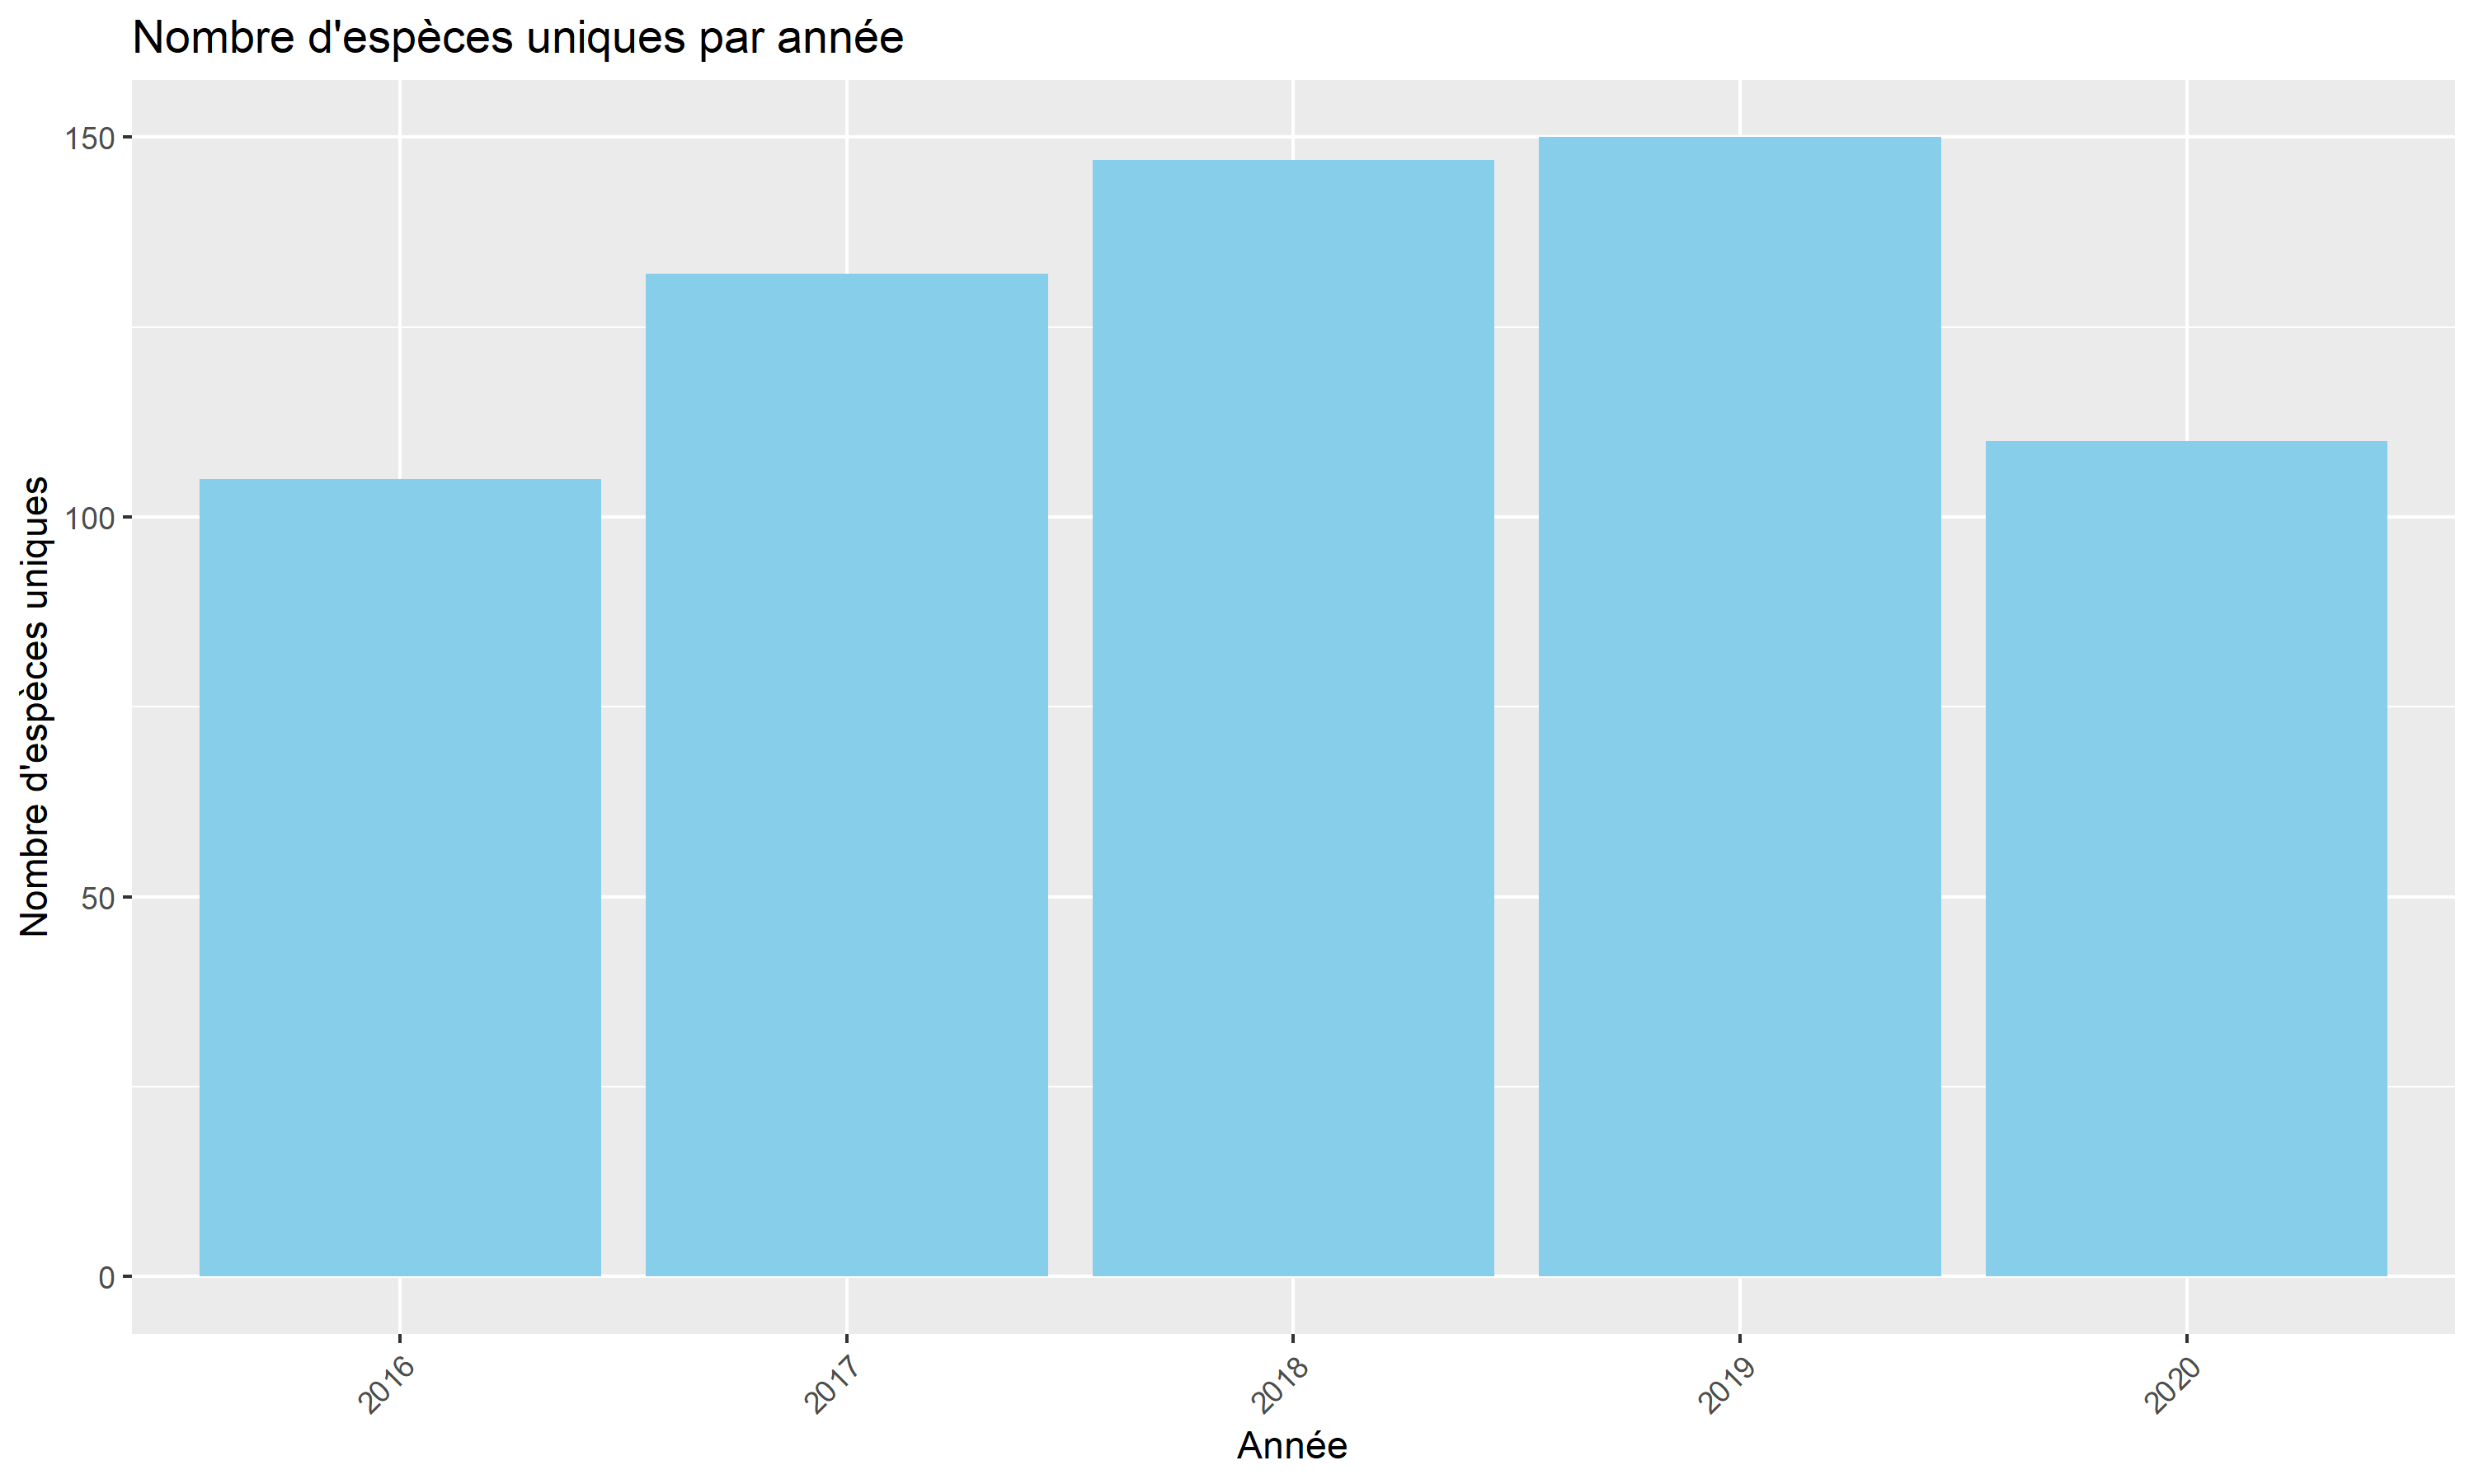
\includegraphics{./rapport/Fig3.png}
\caption{Figure 3: Nombre d'espèce uniques de tous les sites par année}
\end{figure}

\begin{figure}
\centering
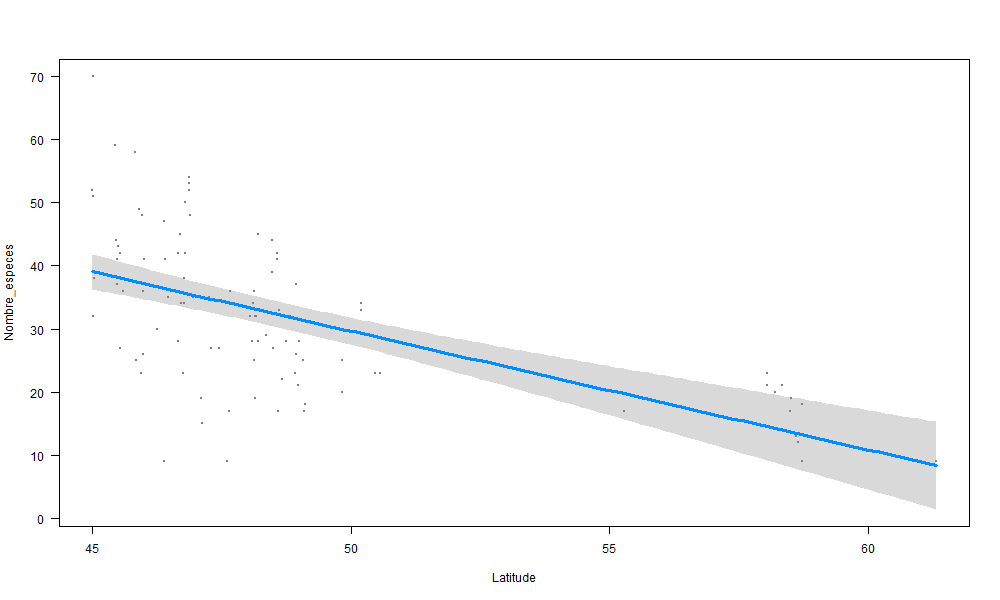
\includegraphics{./rapport/Figure4.png}
\caption{Figure 4: Nombre d'espèce uniques de tous les sites par année}
\end{figure}

\begin{center}\rule{0.5\linewidth}{0.5pt}\end{center}

======= \showmatmethods \showacknow \pnasbreak =======

\end{document}
